\section{Unifying Caches and TLBs}
\label{sec:UCAT}

\noindent Modern chip multiprocessors use multi-level TLB and cache
hierarchies for high performance. The last-level in each hierarchy is
architected as a single large unified structure that holds both
instruction and data entries and is shared among all cores. For
example, the unified last-level cache (LLC) contains hundreds of
thousands of cache lines\footnote{An 8MB cache with 32B lines contains
256K cache lines.}. Similarly, the unified last-level TLB (LLT)
contains 512-1024 TLB entries~\cite{}.

% that store data for recent memory references.
% that store address translations for recent memory references.

The LLT and LLC are cache structures with a tag array and a data
array. The LLT tag array stores virtual addresses while the LLC tag
array stores physical addresses.\footnote{Additional meta data (e.g.
coherence state, replacement state, etc) is also stored in the tag
array.}. The LLT data array stores the physical address corresponding
to the virtual address translation (roughly 8 bytes), while the LLC
data array stores a copy of the data from memory at a cache line
granularity (e.g. 32-64 bytes).

The LLT and LLC caches have similar sized tag arrays. Since they
provide different types of data however, the LLC has a 4x-8x larger
data array. Because of this, the LLC could potentially also serve as
gigantic TLB with as many entries as there are LLC lines.
%EIMAN-03-21: verify that each LLC line can indeed hold one LLT entry.
As such, given that last-level caches typically do not get very high
hit-rates and are often inefficiently used~\cite{}, the conventional
LLC can potentially be used to store virtual to physical translations
just like a TLB in addition to caching data from memory. Based on this
insight, we propose to re-architect the conventional LLC as a {\em
Unified Cache and TLB (UCAT)}.

\begin{figure*}[tbh] 
\vspace{-0. in}
\centering
\centerline{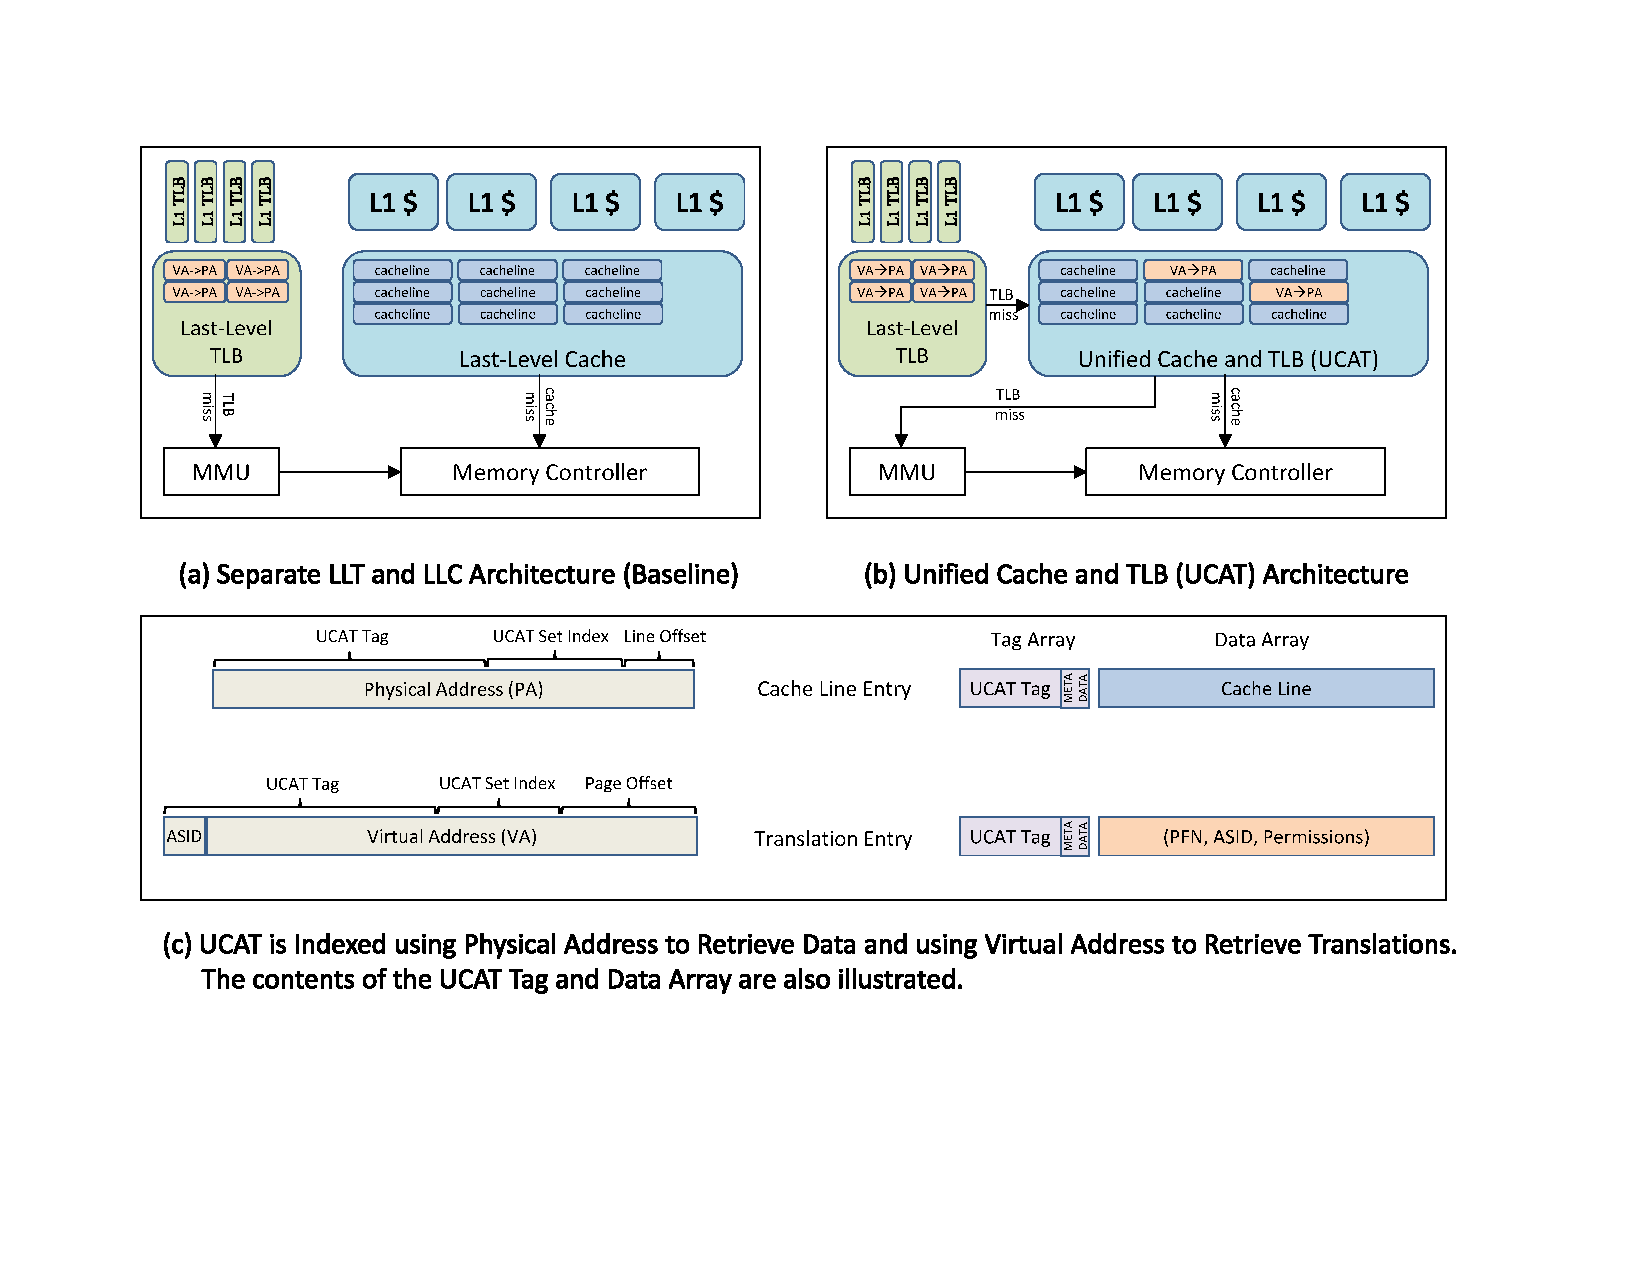
\psfig{file=FIGURES/UCAT,scale=0.80,width=\textwidth}}
\caption{\small UCAT Architecture. \normalsize}
\label{fig:UCAT} 
\vspace{-0.0in}
\end{figure*}

%EIMAN-03-21: My summary for reworking later: 
%   - both TLB and cache hierarchies involve multiple levels and many entries in the unified LL
%   - there is a distinction between what the tag and data of each hierarhcy holds but the cache data portion is bigger
%   - Since the tag arrays are similar in size (does this even matter?), we think of using part of the larger part of the data array of the caches to hold translation entries?
%   - Could the motivaiton here at the end be done better? Isn't the motivation really that the LLC space isn't very efficiently used in the GPU, and its the GPU translations that we care about based on the citation that we had in the intro, right?

\subsection{UCAT Architecture}

\noindent Figure~\ref{fig:UCAT}(a) illustrates a baseline system with
separate LLT and LLC structures, while Figure~\ref{fig:UCAT}(b)
demonstrates a Unified Cache and TLB (UCAT) which holds both cache
lines and TLB entries in a single hardware structure. In the latter, a
UCAT-entry is either a cacheline or a TLB-entry as determined by a
single bit in each UCAT entry. Figure~\ref{fig:UCAT}(c) shows how this
is done. When a UCAT entry stores a cache line similar to what the
baseline system does, the tag-array stores a portion of the physical
address while the data array stores the cache line (e.g.
32-bytes)~\footnote{In our baseline we assume a physically indexed,
physically tagged cache. However, any other variant of virtual or
physical indexing/tagging is equally possible with a UCAT.}. However,
when the UCAT entry serves as a TLB entry, the UCAT tag-array stores
portions of the virtual address and the address space identifier
(ASID) while the data-array stores the virtual to physical address
translation. We propose to use 16 bytes of the UCAT data array for
address translation. In addition to the physical address, the
UCAT-entry also stores meta-data information such as page protection
bits and the LSB of the ASID bits\footnote{When the ASID bits do not
fit in the existing LLC tag array size, we use the MSB of the ASID for
a partial tag match in the tag array. The LSB of the ASID stored in
the data array is then used to finish the tag match before supplying
the stored address translation}.

Note that even though we only use 16-bytes to store the translation,
we do not think we are introducing any new inefficiency. This is
because many recent studies have shown (and independently verified in
this study) that the majority of LLC entries are unused after cache
insertion~\cite{}. In other words, we find that UCAT utilizes the
conventional LLC space more efficiently by storing TLB entries in
addition to cache lines.

% \subsection{Static UCAT Partitioning}
% 
% \noindent UCAT entries must be distributed between TLB-entries and
% cachelines. One way of accomplishing this is by statically employing
% {\em way partitioning}~\cite{}. With {\em N} ways in a UCAT set, {\em
% m} ways are statically devoted to cachelines while the remaining {\em
% N-m} ways are statically devoted to TLB entries. Cachelines are only
% inserted in the ways to devoted to them while TLB entries are inserted
% in the ways devoted to them. When evicting UCAT entries, a replacement
% policy is used (e.g. LRU, RRIP) to select between candidates within
% the same UCAT partition. We refer to this design as {\em Static UCAT
% Partitioning (UCAT-S)}.
% 
% Profiling across various workloads for different values of {\em m} can
% help arrive at the best UCAT partition for cachelines and TLB entries.
% Figure X illustrates the behavior for different {\em m}.

\subsection{UCAT Allocation and Management}

% PUCAT is inefficient when the TLB-entries and cachelines have
% different capacity requirements at run time. To address this problen,

TLB-entries and cachelines dynamically share entries in a UCAT set and
contend with one another for UCAT space. Similar to the baseline, a
single replacement policy is used to manage UCAT entries in a set.
UCAT hits update the replacement state appropriately while UCAT misses
utilize the conventional replacement policy to select the victim
candidate within the set. Figure Y shows UCAT performance.

The baseline UCAT allocates entries based on demand, rather than
utility. As such, workloads that frequently stream through a large
number of cache lines can constantly discard UCAT TLB entries. Based
on this observation, we enhance UCAT by improving the underlying UCAT
replacement policy. To this end we use the Dynamic Re-Reference
Interval Prediction (DRRIP) replacement policy~\cite{}. In this
policy, all UCAT insertions follow the same re-reference prediction
(i.e. insertion policy). We propose to enhance the insertion policy
for TLB entries by inserting them with a {\em near-immediate
prediction} rather than the default {\em far prediction}. In doing so,
TLB entries are allowed to reside in the UCAT for a longer duration.
We refer to this enhancement as {\em UCAT with Insertion (UCAT-I)}.

Figure Y also shows performance of UCAT-I.

\begin{figure*}[t] 
  \vspace{-0. in} \centering
%  \centerline{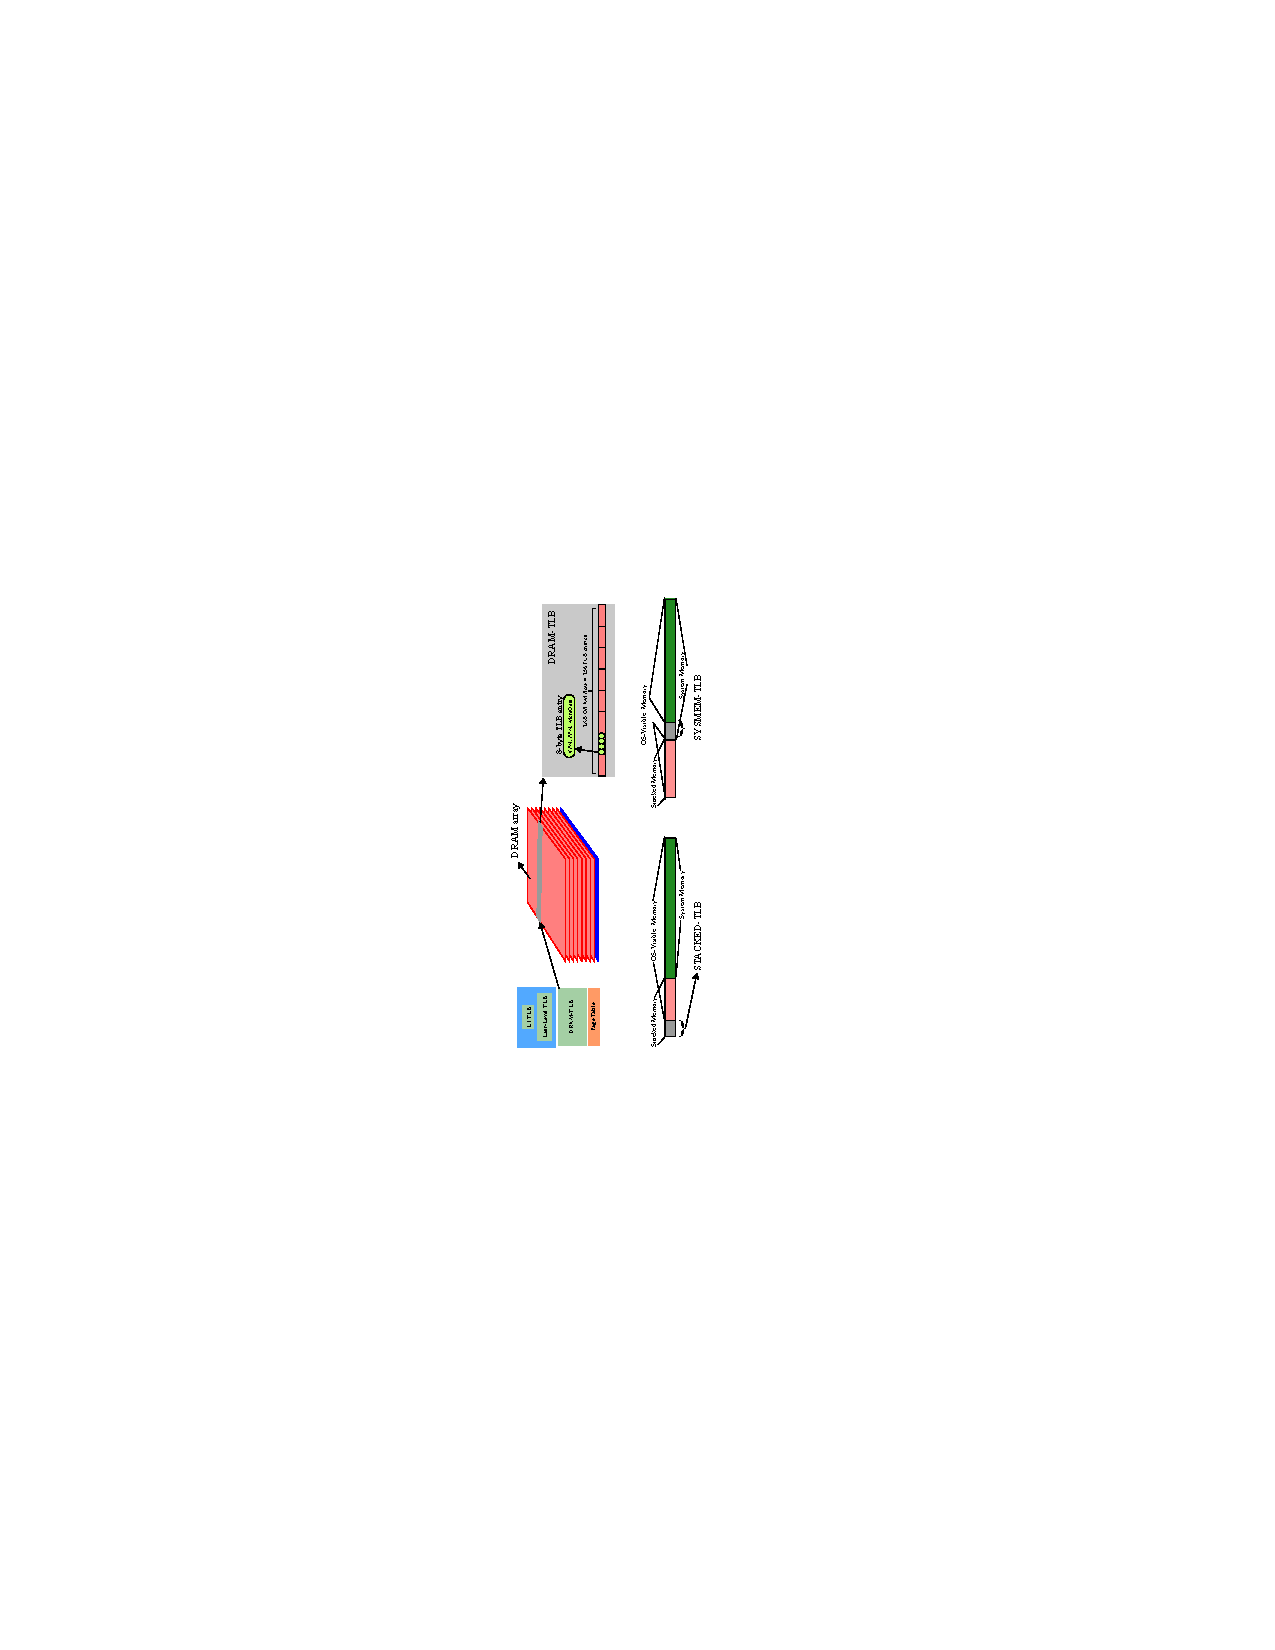
\psfig{file=FIGURES/stacked_tlb,angle=-90,width=\columnwidth}}
   \centerline{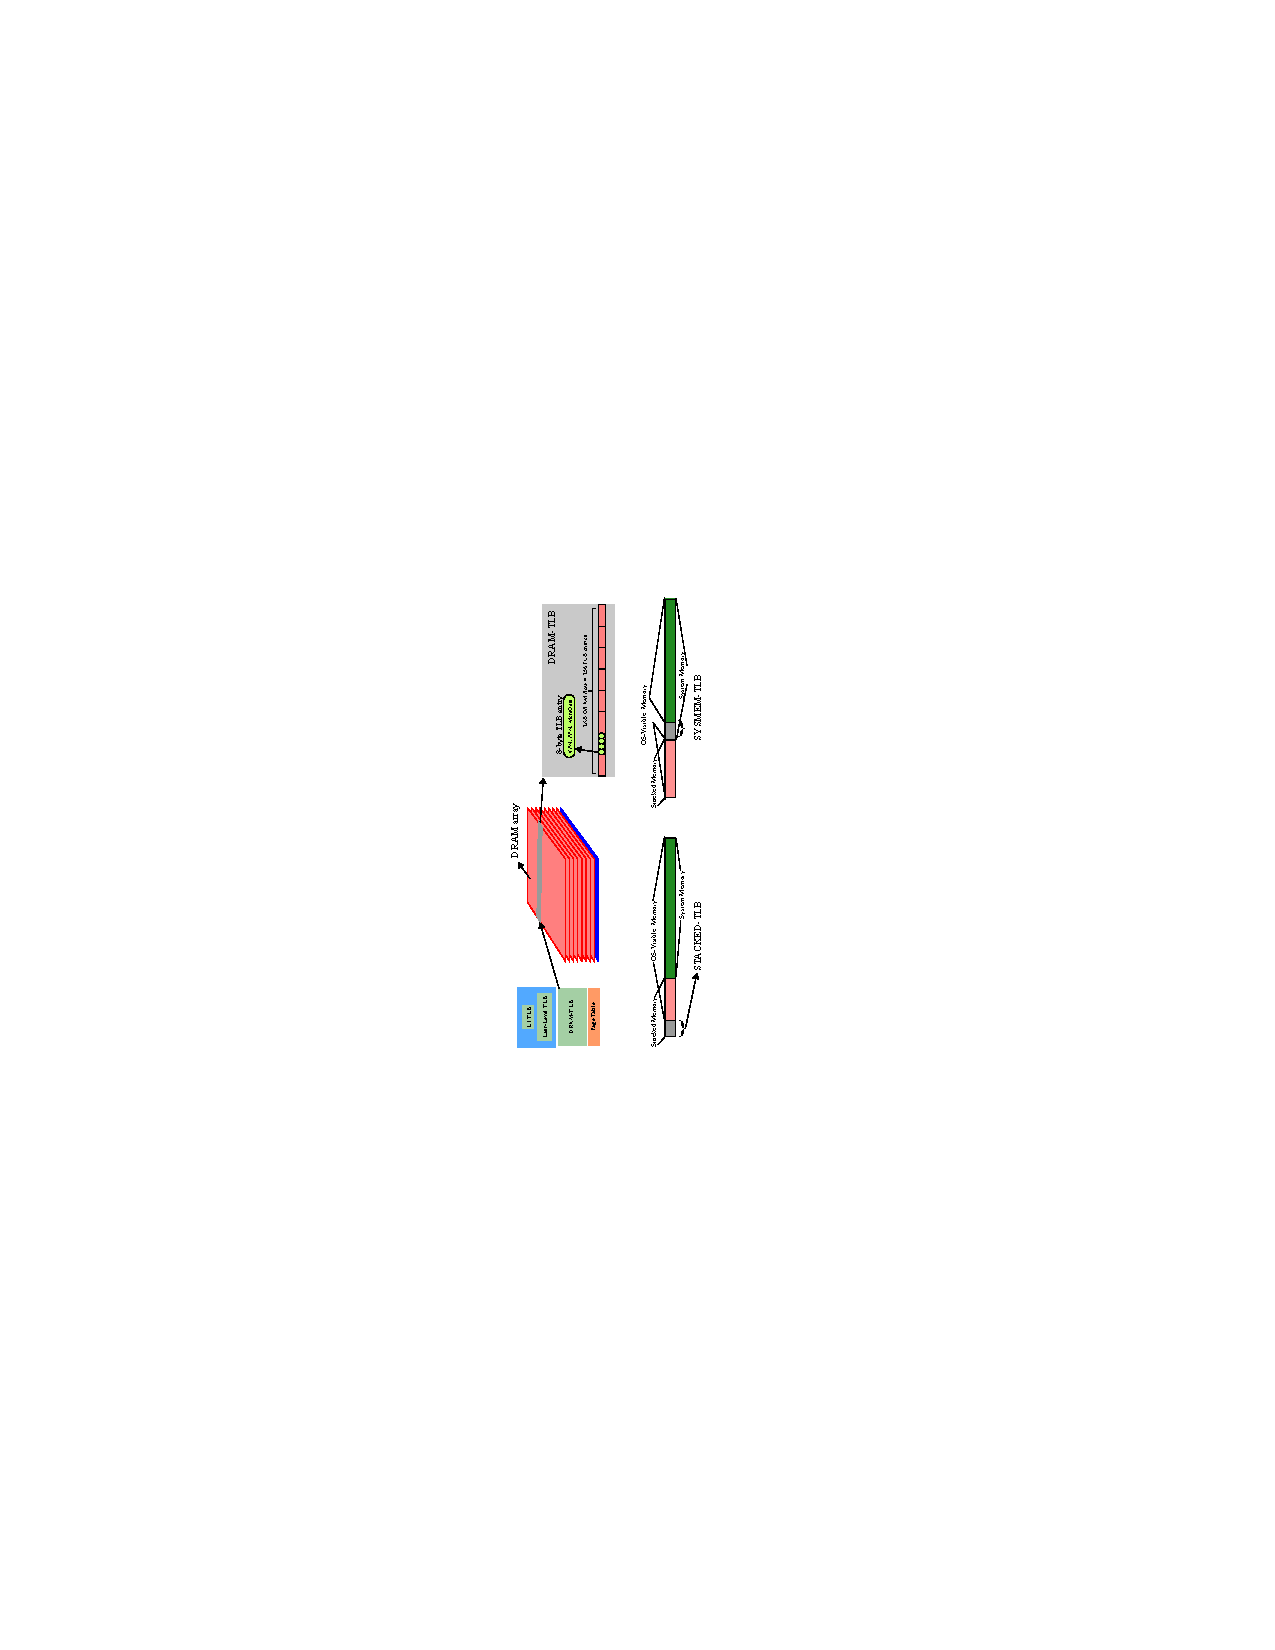
\psfig{file=FIGURES/stacked_tlb,width=\textwidth}}

  \caption{\small Improving TLB coverage by embedding TLBs in DRAM
    (DRAM-TLB). A DRAM-TLB architected using commodity DRAM is called
    SYSMEM-TLB and a DRAM-TLB architected with stacked DRAM is called
    Stacked-TLB. \normalsize}
  \label{fig:stacked_tlb} 
  \vspace{-0. in}
\end{figure*}

\begin{figure}[tp] 
  \vspace{-0.in} \centering
  \centerline{\psfig{file=GRAPHS/UCAT_perf,angle=-90,width=\columnwidth}}

  \caption{\small Performance of DRAM-TLBs. \normalsize}
  \label{fig:perf_UCAT} 
  \vspace{0.2 in}
\end{figure}

\begin{figure}[tp] 
  \vspace{0.in} \centering
  \centerline{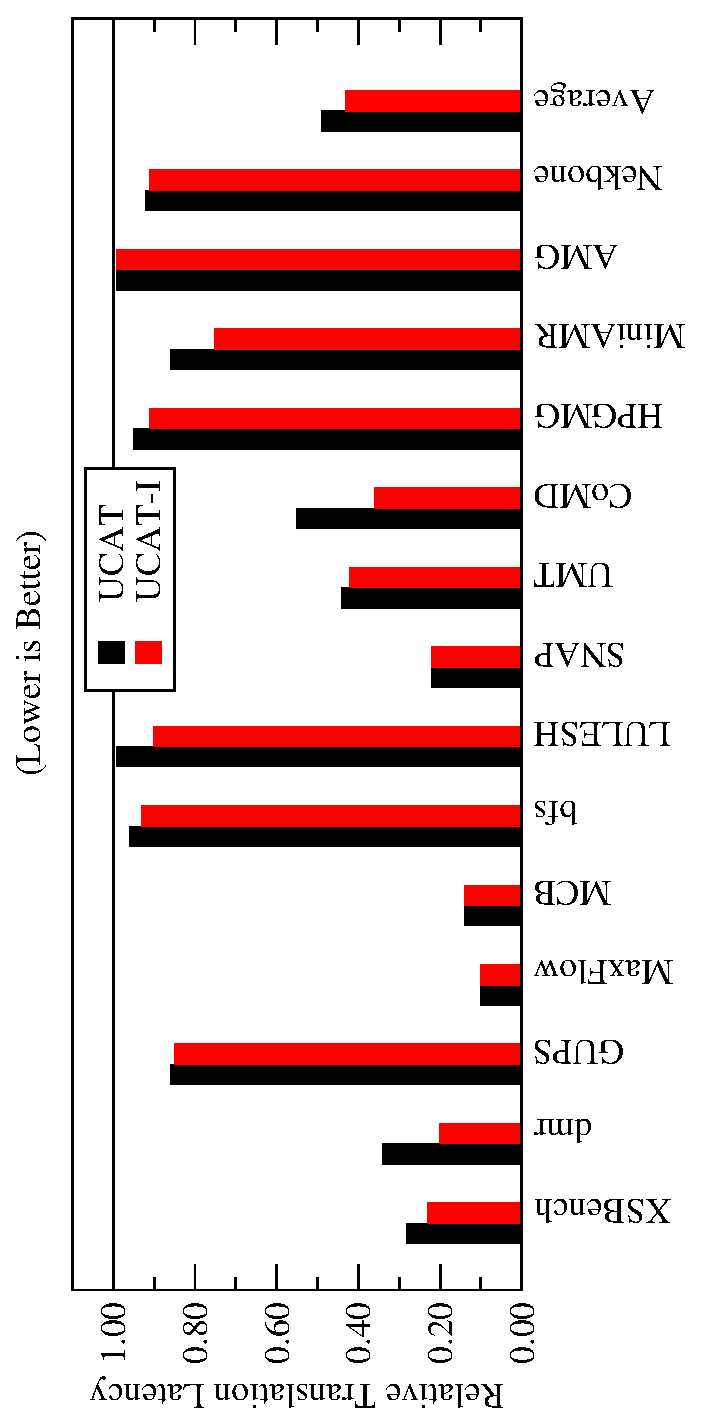
\psfig{file=GRAPHS/UCAT_tlblat,angle=-90,width=\columnwidth}}

  \caption{\small TLB miss penalty relative to baseline system.\normalsize}
  \label{fig:tlblat_UCAT} 
  \vspace{-0.1 in}
\end{figure}

\begin{figure}[tp] 
  \vspace{0.in} \centering
  \centerline{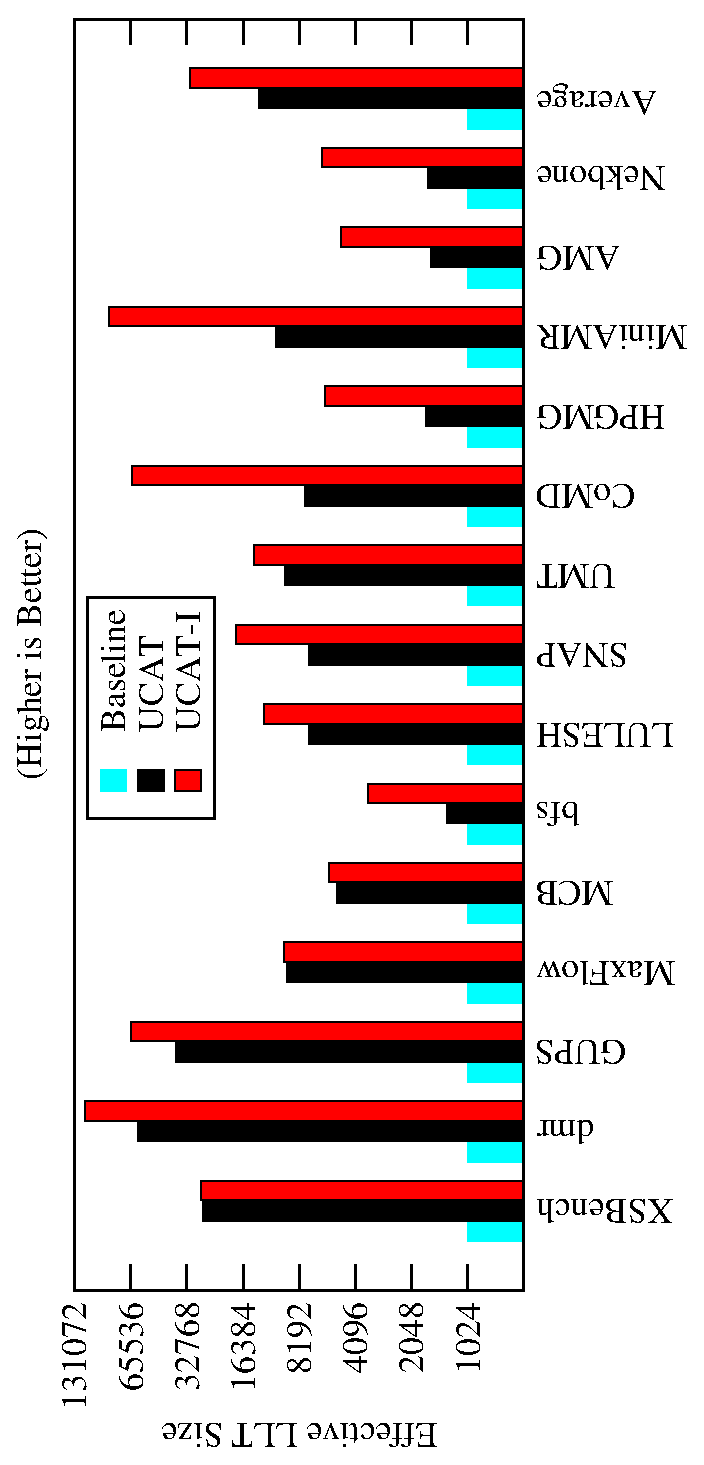
\psfig{file=GRAPHS/UCAT_tlbsize,angle=-90,width=\columnwidth}}

  \caption{\small Effective TLB Size.\normalsize}
  \label{fig:tlblat_UCAT} 
  \vspace{-0.1 in}
\end{figure}


\subsection{UCAT Optimizations}

To avoid any additional storage overhead, we propose using the
UCAT-entry status bits (i.e., MESI bits) to make the distinction between 
a cache-line entry and a translation entry in the UCAT.
Specifically, we insert TLB-entries into UCAT with the {\em exclusive}
and {\em shared} status bits both set to valid. Note that cachelines can
either be in exclusive state or shared state, but not both.

